\chapter{GAT-Denoiser}
\label{sec:contribution}

In this Chapter, I introduce my methodological approach.
As a result, a GNN is derived which is called \textit{GAT-Denoiser}.
Its main components and overall architecture is introduced.


\paragraph{Goal:}
As introduced in Chapter~\ref{sec:imaging} \textit{\nameref{sec:imaging}}, molecular imaging methods computed tomography and cryo-EM are the problems
to approach. Further, high-noise regime is the domain of interest, to be more precise SNR between $[-10, 0]$.
For a given set of observations (many sinograms or micrographs), a GNN will be trained, such that
it enables denoising of observations which are expected to have a better reconstruction result after denoising.
Trained model allows to denoise not seen observations which are from the same family of observations.


\begin{tcolorbox}[colback=red!5!white,colframe=red!75!black]
  An algorithm was designed to work with CT, projection angles are assumed to be known and $\theta$ was defined as equally spaced 
  in the interval $[0, \pi]$. 
\end{tcolorbox}

\paragraph{Input graph:}
To recap from Section~\ref{sec:graphConstruction}  \textit{\nameref{sec:graphConstruction}}, 
a graph constructed from molecular-imaging observation will have single observations as nodes (one horizontal line of the sinogram). 
As $\theta$ is fixed, angle corresponding to each single observation are known. 
Based on these angles, neighboring nodes can be connected.

\begin{tcolorbox}[colback=red!5!white,colframe=red!75!black]
  For GAT-Denoiser, this entails that graph topology is fixed and
  a k-NN graph can be constructed from $\theta$.
\end{tcolorbox}


\textbf{TODO: Change title name}

\section{Concept}
\label{sec:concept}

In the following section, the concept of GAT-Denoiser is introduced. 
GAT-Denoiser is a GNN and has two main components, namely convolution layers and GAT layers.
The main idea of GAT-Denoiser is to enable denoising of observations:
\begin{equation}
  \textit{GAT-Denoiser} (\cdot) : L^2(\tilde{\Omega}) \to  L^2(\tilde{\Omega}) , y \mapsto \textit{GAT-Denoiser} (y) 
\end{equation}

% The GAT is expected to denoise observation signal with its neighbours by averaging. 
% Further, convolution is added to denoise single observations.

Input $y$ of GAT-Denoiser is a noisy observation, output is a denoised version.
GAT averages over observation neighbors and convolution to denoise single observations. 
For every GAT layer there is a preceding convolution. 
In the case of computed tomography, convolution is in 1D, where for cryo-EM in 2D.

\begin{tcolorbox}[colback=red!5!white,colframe=red!75!black]
  The GAT denoise observation signal with its neighbors by averaging. 
  Further, convolution is added to denoise single observations.
\end{tcolorbox}


But, the main overall goal is to get the best possible reconstruction 
from noisy observation $y$ which approximates original object $x$ and 
not just denoise observation $y$ which approximates noiseless observation $p$.


\begin{equation}
  \begin{aligned}
    x \approx   &\textit{Recon} \left( \textit{GAT-Denoiser} \left( y \right) \right), \\
    \text{with } &\textit{Recon} : \textit{UNet} \left( \textit{FBP} \left( \cdot \right) \right)  
  \end{aligned}
\end{equation}

Therefore, an end-to-end learning approach is used where quality of reconstruction is 
compared during GAT-Denoiser training, which is expected to perform better than 
only optimizing denoising of observations.

In Figure~\ref{fig:overall-concept} overall GAT-Denoiser concept is illustrated.
\begin{figure}[H]
  \centering
  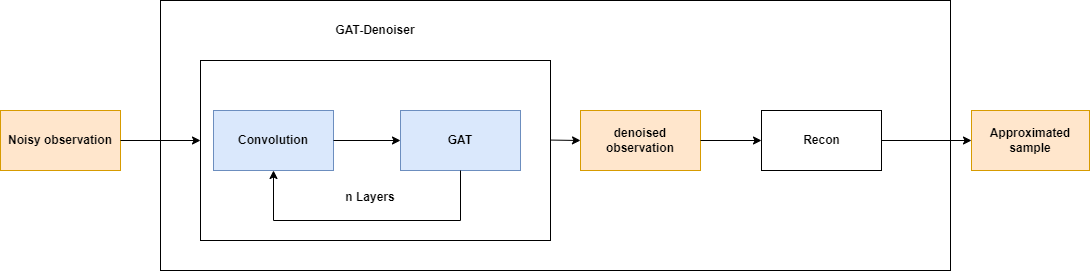
\includegraphics[width=\textwidth]{Overall_GAT-Denoiser_Pipeline.drawio.png}
  \caption{GAT-Denoiser concept}
  \label{fig:overall-concept}
\end{figure}



\paragraph{K-hop neighborhood:}
In GNNs, multiple layers expose the k-hop neighborhood. So for a network with $k$ layers,
network operates on the $k$-hop neighborhood. In GAT-Denoiser, this corresponds
to the layers of GAT. Therefore, if writing from one layer, it is referring to convolution and GAT together.

\section{Components}
In this section, the three components are introduced individually.

\subsection{Graph Attention Networks}
The main component of GAT-Denoiser is a GAT.
As mentioned in Section~\ref{sec:graph_depp_learning} \textit{\nameref{sec:graph_depp_learning}}, GAT is an extension to GCN and 
adds attention (or weights) to neighbors for learning new node feature representations. 
Again, topology of the graph will not change but weighted averaging over the neighborhood 
will take place and this is what in denoising is a good idea.

\paragraph{Single Layer}
Input of a single GAT layer are node features $h = \{ h_1, h_2, \dots , h_N \} \in \mathbb{R}^F$, 
where $N$ is the number of nodes and $F$ the number of features per node. 
Single layer will map input to output, which can potentially have different dimensions: 
$h^{\prime} = \{ h_1^{\prime}, h_2^{\prime}, \dots, h_N^{\prime} \} \in \mathbb{R}^{F^{\prime}} $
As is other GNNs, input features are initially linearly transformed and parametrized by a learnable weight matrix 
$W \in \mathbb{R}^{F^{\prime} \times F}$. 
This allows to add enough expressiveness to the neural network and weights are learned during training.
Further, attention coefficients are computed, which indicates importance of node $j$ to node $i$:

\begin{equation}
  e_{ij} = a(Wh_i, Wh_j)
\end{equation}

With $a$ as the shared attentional mechanism $a : \mathbb{R}^{F^{\prime}} \times \mathbb{R}^{F^{\prime}} \mapsto \mathbb{R}$.
\citet{GAT} proposed to use a single-layer feedforward neural network, parametrized by a weight vector $a \in \mathbb{R}^{2F^{\prime}}$
and LeakyReLu as activation function.

To compare coefficients $e$ across different nodes, normalization is needed.
Therefore, softmax is used as normalization $\alpha_{ij} = softmax_j(e_{ij})$ 
such that all attention coefficient of one node sum up to 1 and therefore are nicely comparable across nodes.
Finally, new node embedding is calculated as:

\begin{equation}
  h_i^{\prime} = \sigma \left( \sum_{j \in \mathcal{N}_i} \alpha_{ij} W h_j \right)
\end{equation}

With $\sigma$ as some arbitrary activation function.

\paragraph{Multi-Head attention}
Motivated by the work of \citet{transformer}, multi-head attention can be beneficial to stabilize learning process.
Therefore, not only a single weight matrix is learned, but $W$ is split up in several parts, 
all learned individually:

\begin{equation}
  h_i^{\prime} = \bigparallel^K_{k=1} \sigma \left(\sum_{j \in \mathcal{N}_i} \alpha_{ij}^k W^k h_j \right),  
\end{equation}

Where $\parallel$ corresponds to concatenation, $\alpha_{ij}^k$ the $k$-th attention mechanism and $W^k$ the linear
transformations weight matrix. The final output consists of $KF^{\prime}$ output features.

\paragraph{Last layer:}
In the last layer, output dimension needs to be obtained. 
Consequently, concatenation is no longer plausible and averaging is used to match desired dimension.

\subsection{Convolution}
The second key component of GAT-Denoiser is convolution.
Convolution is an important part in Signal Processing, because it allows to average an incoming signal.
Convolution commonly operators on pixel spaces, where every observation location or time slot gets one value assigned.

\begin{equation}
  x \star k = y,
\end{equation}

Where $x$ is input signal, $k$ is kernel, $\star$ the convolution operator and $y$ the convolved signal.

To apply convolution, a kernel with weights needs to be defined. 
This kernel will then slide over the input signal $x$ and computes the dot product with its weights.
In Figure~\ref{fig:1d-convolution} an illustration of 1D convolution can be seen. In this example,
kernel size is set to 3, $n$ refers to input signal dimension and $m$ to output signal dimension.
In the example  $ n = m + 2$, so the convolved output signal will be decreased by $2$.
The concept of convolution can be extended to arbitrary dimensions.

\begin{figure}[H]
  \centering
  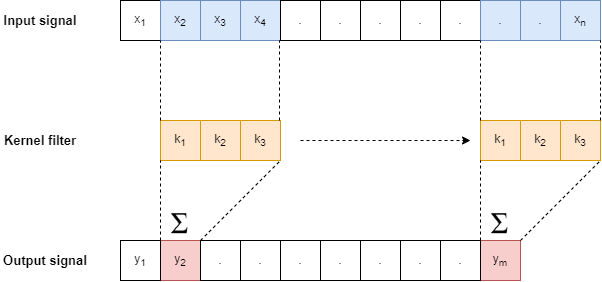
\includegraphics[width=0.6\textwidth]{Convolution.drawio.png}
  \caption{1D Convolution}
  \label{fig:1d-convolution}
\end{figure}

\paragraph{Padding:} 

\textbf{TODO: Replace dimension with signal size}
Padding can be defined to add pixels to boundary of the signal.
In the example, padding is set to $0$ and therefore, the signal dimension is decreased by $2$.
If signal dimension should be fixed during convolution, padding is a powerful tool. For padding $1$,
the input dimension $n$ would be equal to output dimension $m$, as an extra element in the output signal
will be at convolved at boundaries.


\paragraph{Stride:}
Stride is the parameter how far kernel moves each time. In the example, stride was defined to be $1$.
If stride is increased, the output signal dimension will decrease.


\subsection{U-Net}
\label{sec:unet}
U-Net can boost performance of CT reconstruction and is therefore the third component
in GAT-Denoiser.
It is a convolutional neural network, which is well suited for image segmentation in different domains.
\cite{unet-tomography} showed great success for biomedical image segmentation.

The neural network architecture consists of contracting path and expansive path,
resulting in a U-shape, as illustrated in Figure~\ref{fig:u-net-architectue}.

\begin{figure}[H]
  \centering
  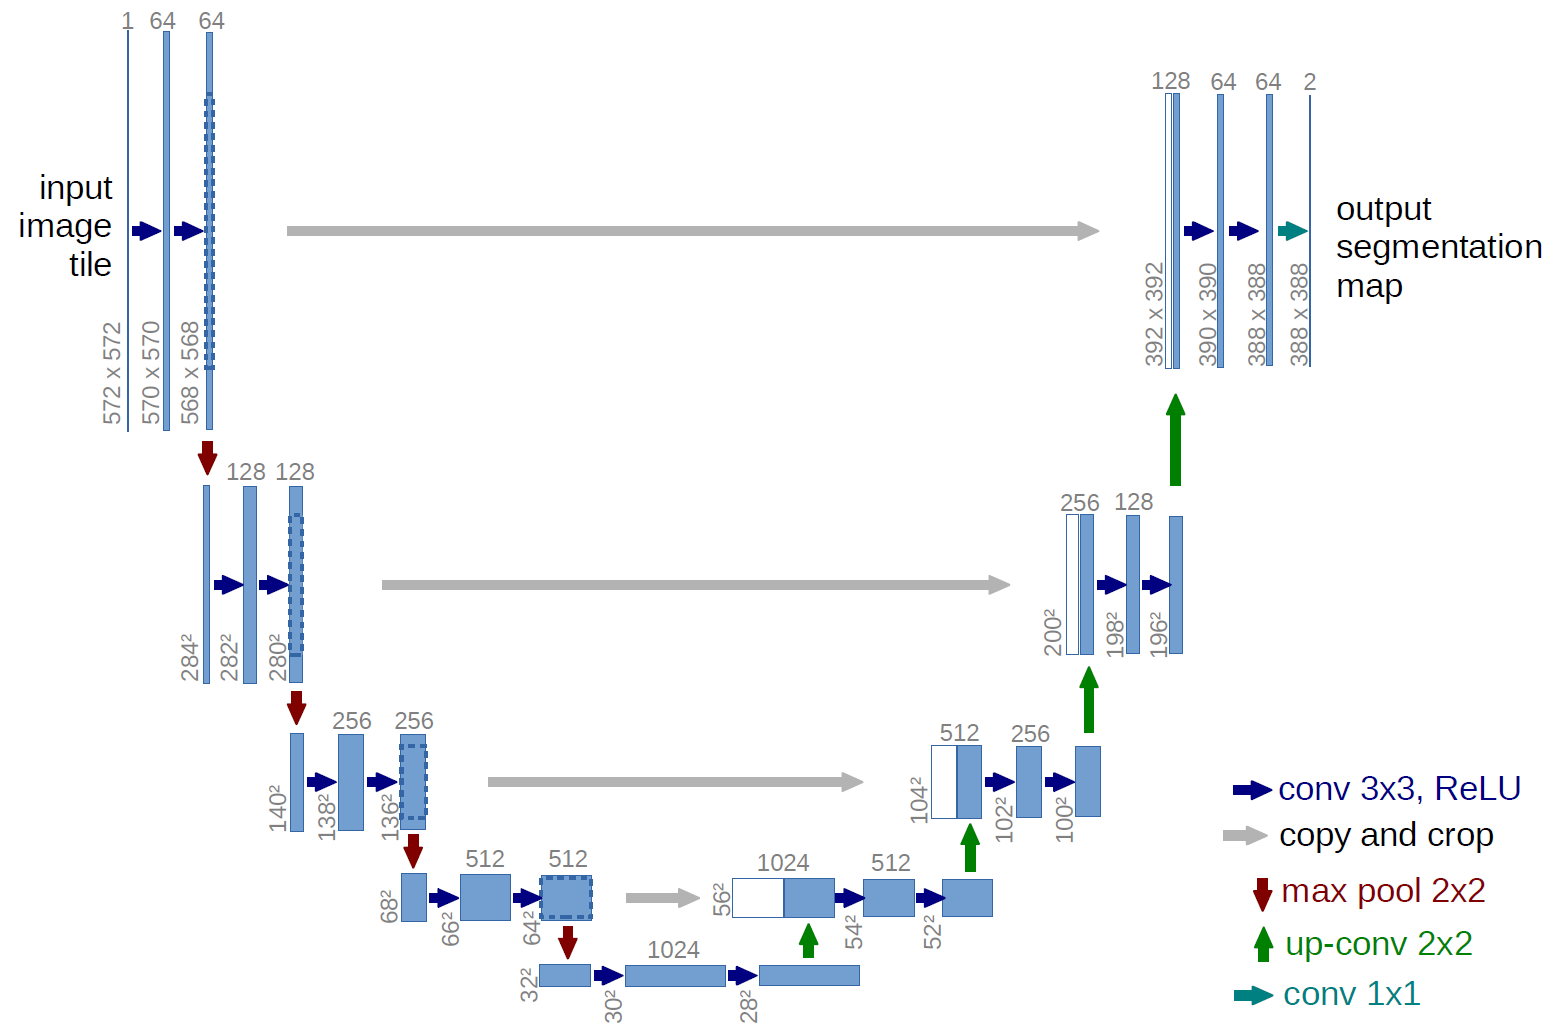
\includegraphics[width=0.6\textwidth]{u-net-architecture.png}
  \caption{
    U-Net architecture \cite[p 2, Fig. 1]{unet-tomography} \\
    Number on top of boxes denotes channels, where numbers at bottom of boxes refer to input dimension.
    }
    \label{fig:u-net-architectue}
\end{figure}


During contracting path (left part), input dimension is decreased but channels increased.
For every step in the contracting path, two 3x3 convolution layers are followed by ReLu
and a 2x2 max pooling for down-sampling. Further, at each down-sampling step, input channels are doubled.
Multiple contracting steps are combined. After last contracting step, expansive path (right part) starts
where input dimension will be increased and input channels will be decreased.
For every expansive step, an up-sampling of the feature map takes place, followed by a 2x2 convolution, 
which halves the number of channels. Then, concatenation with the corresponding feature
map of the contracting path is done (gray arrow in Figure~\ref{fig:u-net-architectue}), followed by again two 3x3 convolutions and ReLu.
Final layer is a 1x1 convolution to map to desired output dimension and single output channel.

\section{Architecture}
\label{sec:architecture-GatDenoiser}
All individual components are introduced and GAT-Denoiser architecture can be defined.
First, the neural network layers will be explained and, second, loss and training.

As defined in Equation~\ref{eq:abstract-model}, $N$ is the number of observation and
$M$ observation dimension. 
Therefore, input (noisy sinogram) will be in $\mathbb{R}^{N \times M}$ as well as output (denoised sinogram). 

\subsection{Layers}
In Figure~\ref{fig:architecture-detailed}, detailed GNN architecture can be seen.
It is parametrized with $channels$, $heads$ and $layers$. 
The number of channels in convolution can be increased with parameter $channels$.
Further, $heads$ determine the number of heads used in the GAT layers and parameter 
$layers$ defines how many convolution and GAT layers are stacked together.

\textbf{TODO: In figure everything bold! Replace parameters with c, h and l?}

\begin{figure}[H]
  \centering
  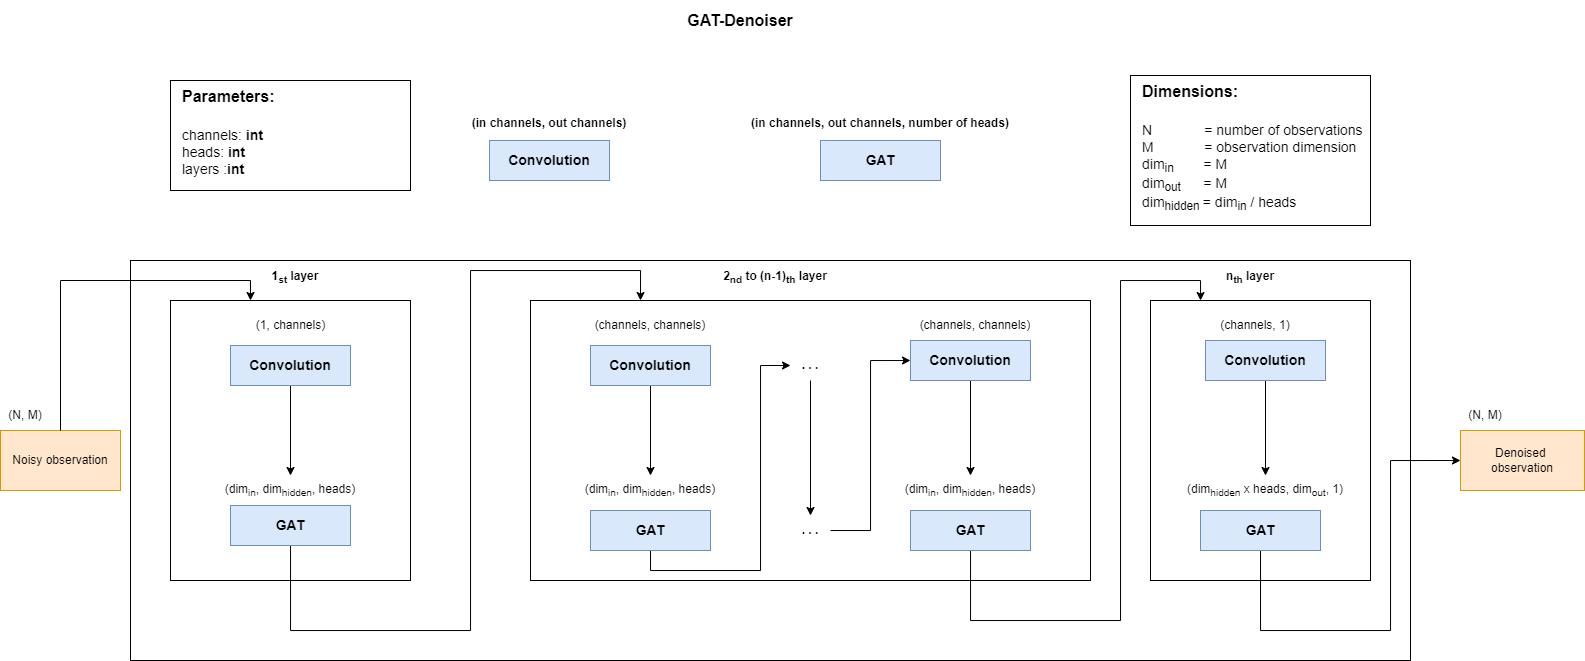
\includegraphics[width=\textwidth]{GAT_Architecture_Detail.drawio.png}
  \caption{Overall GAT-Denoiser architecture}
  \label{fig:architecture-detailed}
\end{figure}


For every layer, first convolution and then GAT is processed. 
Convolution in the whole network was defined with kernel size of 3 and padding 1,
therefore, dimension of convolved signal will not change. 
Convolution can be defined with different parameters, but output signal needs to have 
same dimension as input signal.
Further, additional convolutional channels can be used for learning.
If parameter $channels > 1$, channels are increased in the first convolution layer 
and decreased in the last one.
Parameter $heads$ controls multi-head approach for GAT. Input and hidden dimension
of GAT is $M$ if no heads are used.
If multi-head attention is used, hidden dimension will be set to $M / heads$.
In the last GAT layer, everything gets prepared for output dimension and 
averaging with 1 head is applied.

\subsection{Training}
\label{sec:contr_training}
An end-to-end learning approach is used where quality of reconstruction is 
compared in the loss.

Therefore, the outcome of GAT-Denoiser is not directly part of the loss, but first reconstruction will be computed.
Reconstructions can be nicely compared with the $\ell2$-norm:

\begin{equation}
  \label{eq:loss_reco}
  \mathcal{L} = \parallel x_i - \textit{Recon} ( \textit{GAT-Denoiser}(A(x_i, \theta, s) + \eta)) \parallel ^2_2
\end{equation}

As $x_i$ is part of the loss, access to original object is needed during training.

Further, U-Net will be jointly used with FBP as reconstruction. 
Thus, U-Net needs to be first pre-trained with the dataset.
One could also consider training U-Net and GAT-Denoiser jointly.

\textbf{TODO: Add Loss section with part from second loss.}
